\documentclass[10pt]{article}
\usepackage{graphicx}
\usepackage[margin=1.5cm]{geometry}
\usepackage{amsmath}
\def\brcurs{{\mbox{$\resizebox{.16in}{.08in}{
\includegraphics{BoldR}}$}}}
\def\rcurs{{\mbox{$\resizebox{.16in}{.08in}{
\includegraphics{ScriptR}}$}}}

\begin{document}
\twocolumn

\title{Thursday Warm-up: Amp\`{e}re's Law}
\author{Prof. Jordan C. Hanson}

\maketitle

\section{Memory Bank}

\begin{itemize}
\item \textbf{The Biot-Savart Law}, for steady currents:
\begin{equation}
\mathbf{B}(\mathbf{r}) = \frac{\mu_0 I}{4\pi}\int \frac{d\mathbf{l}'\times \hat{\brcurs}}{\rcurs^2}
\end{equation}
\item \textbf{Amp\`{e}re's Law}, differential form:
\begin{equation}
\nabla \times \mathbf{B} = \mu_0 \mathbf{J}
\end{equation}
\item \textbf{Amp\`{e}re's Law}, integral form:
\begin{equation}
\oint \mathbf{B} \cdot d\mathbf{l} = \mu_0 I_{\rm enc}
\end{equation}
\end{itemize}

\begin{figure}
\centering
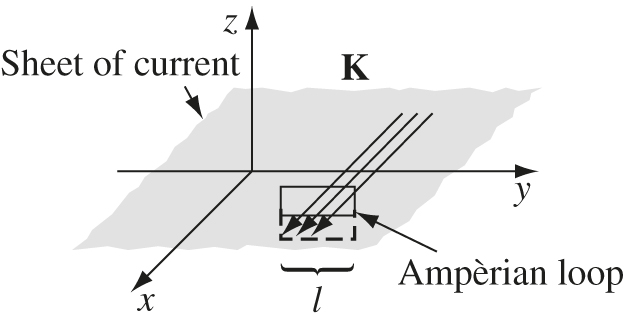
\includegraphics[width=0.35\textwidth]{figures/5_32.jpg} \\ \vspace{0.5cm}
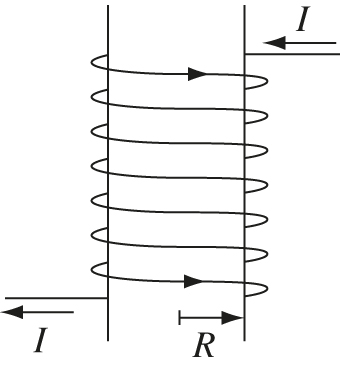
\includegraphics[width=0.175\textwidth]{figures/5_33.jpg} \hspace{0.5cm}
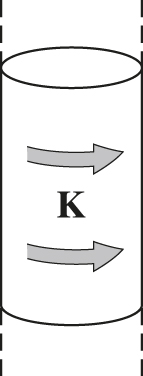
\includegraphics[width=0.075\textwidth]{figures/5_34.jpg} \\
\caption{\label{fig:1} (Top) A sheet of current, $\mathbf{K} = K\hat{\mathbf{x}}$. (Bottom left) A solenoid with finite windings.  (Bottom left) A solenoid with high density of windings.}
\end{figure}

\section{Amp\`{e}re's Law}

\begin{enumerate}
\item Consider Fig. \ref{fig:1} (top).  Find the $\mathbf{B}$-field the surface current $\mathbf{K} = K\hat{\mathbf{x}}$, flowing in the $xy$-plane. (a) First, identify the \textit{direction} of the field, above and below the sheet.  Second, calculate the \textit{magnitude} of the field. (b) In which direction would a small current in the +$x$-direction above the sheet move? What about a small current in the +$x$-direction below the sheet? \\ \vspace{4cm}
\item Consider Fig. \ref{fig:1} (bottom left and right).  (a) Find the $\mathbf{B}$-field of a very long solenoid, consisting of $n$ closely wound turns per unit length on a cylinder of radius $R$, each carrying a steady current $I$. \textit{Hint: use the Amperian loops in Fig. \ref{fig:2} to establish the field inside and outside of the solenoid}.  (b) Suppose we shoot a beam of positively-charged particles through the solenoid.  Sketch the trajectory of the particles.\\ \vspace{4cm}
\end{enumerate}

\begin{figure}[hb]
\centering
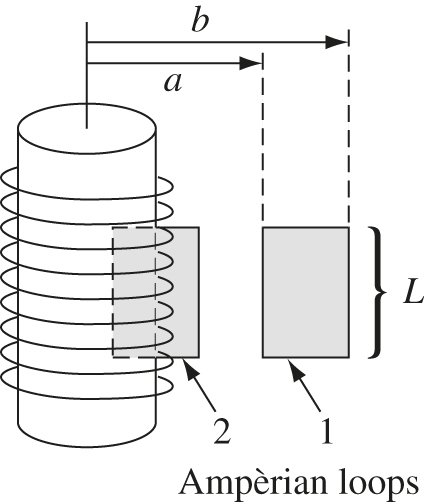
\includegraphics[width=0.25\textwidth]{figures/5_36.jpg}
\caption{\label{fig:2} The Amperian loops used for solenoid calculations.}
\end{figure}

\end{document}
